\subsection{Apparent difficulty and measured contribution move in opposite directions}

Holding the model, the positives, the folds and the estimator fixed and changing only how the
negative windows were built gives three different pictures of the same 4-mer on the same 94
datasets (Table~\ref{tab:three}, Figure~\ref{fig:three}).

\begin{table}[htbp]
\centering
\caption{The same model on the same positives under three negative-set protocols, $n=94$
datasets. Only the construction of the negative windows differs.}
\label{tab:three}
\begin{tabular}{lccc}
\toprule
protocol & composition alone & apparent AUROC & nested contribution \\
\midrule
dinucleotide-matched & 0.6274 & 0.6937 & $+0.0663$ \\
GC-matched & 0.7827 & 0.8092 & $+0.0265$ \\
bias-aware (other RBPs' sites) & 0.8248 & 0.8370 & $+0.0122$ \\
\bottomrule
\end{tabular}
\end{table}

Moving from GC-matched to dinucleotide-matched negatives lowers apparent AUROC by 0.1095, and it
does so in 94 of 94 datasets (paired Wilcoxon $p<10^{-15}$). The same change raises the measured
contribution from $+0.0265$ to $+0.0663$, a contrast of $+0.0398$ $[+0.0325, +0.0477]$
(protein-clustered, positive in 88 of 94). A reader comparing the two benchmarks by headline
AUROC would conclude the model had got worse. A reader comparing what the model added would
conclude it had got nearly three times better. Both readings are correct about their own
quantity, and they point in opposite directions.

The bias-aware protocol is where this becomes a problem for practice. Drawing negatives from
other proteins' binding sites is designed to remove the compositional and accessibility
artefacts that genomic-background negatives carry, and it does: those negatives are transcribed,
crosslink-accessible and strand-correct by construction, and no composition matcher touches
them. We pre-registered the prediction that composition would fall toward 0.5 under this
protocol, because both classes are real crosslink sites, and that the measured contribution
would rise. Both halves were wrong. Composition alone is the \emph{highest} of the three arms at
0.8248, the discrimination is the \emph{easiest} of the three by apparent AUROC at 0.8370, and
the measured contribution is the \emph{lowest} at $+0.0122$, 0.53 times the GC arm (geometric
mean over the 83 datasets positive in both arms; the ratio of panel means is 0.46). The reason is
visible in hindsight and is itself a result: different RBPs bind compositionally different sites,
so telling one protein's sites from another's is largely a composition task.

The ordering is therefore monotone in measured difficulty and not in how principled the protocol
sounds. Ranked by composition alone, by apparent AUROC or by contribution, all three orderings
agree. ``Harder negatives reveal more of what a model adds'' is exactly true. What is false is
the inference that a bias-aware protocol is harder: it is the easiest of the three, and it
reveals the least.

Two further features of Table~\ref{tab:three} matter for interpretation. Composition alone beats
the 4-mer outright in 29 of 94 datasets under GC matching. And the 4-mer's contribution is
significantly positive in 80 of 94 datasets, falling to 72 of 94 at the design effect measured
for these data (Methods), so on roughly a quarter of the panel the model adds nothing detectable
over composition under the protocol in common use.

The \emph{sign} of the GC-versus-dinucleotide contrast is implied by the design, and we state
this here rather than in a limitations paragraph. The composition baseline occupies the fifteen
degrees of freedom of the dinucleotide simplex; GC matching constrains one linear functional of
that space and dinucleotide matching constrains all fifteen, so the arm that controls more of
the baseline must leave the baseline weaker and the model more room. Only the \emph{magnitude}
is informative. What the design does not imply is the bias-aware arm's position: that protocol
constrains \emph{none} of the fifteen degrees of freedom, its negatives are not
composition-matched in any respect (median absolute GC gap 0.1387 against the GC arm's 0.0297),
and it nonetheless has the highest composition baseline of the three. No degrees-of-freedom
argument predicts that, and it is what breaks a purely circular reading of the table.

\paragraph{Artefact controls.} Two alternative explanations were pre-registered and bounded
against matched placebos, each with twenty placebo seeds. A strand-annotation artefact, arising
because a matched negative inherits its positive's strand label, accounts for $-0.0055$
$[-0.0089, -0.0022]$ of the contrast, leaving 85.4\% standing. Negatives drawn from
untranscribed loci account for $-0.0043$ $[-0.0069, -0.0018]$, leaving 89.7\%; 40.1\% of
negatives lie in untranscribed loci, but that fraction is balanced across the two arms to within
$1.2\times10^{-5}$ ($p=0.64$), and a confound present equally in both arms cannot manufacture a
difference between them. One argument needs no placebo: GC-matched negatives are 42.8\% sense
against 47.4\% in the dinucleotide arm, higher in 37 of 40 datasets ($p=5.0\times10^{-9}$), so
the spurious directional cue is stronger in the arm with the \emph{smaller} contribution and
works against the reported direction.

\begin{figure}[htbp]
\centering
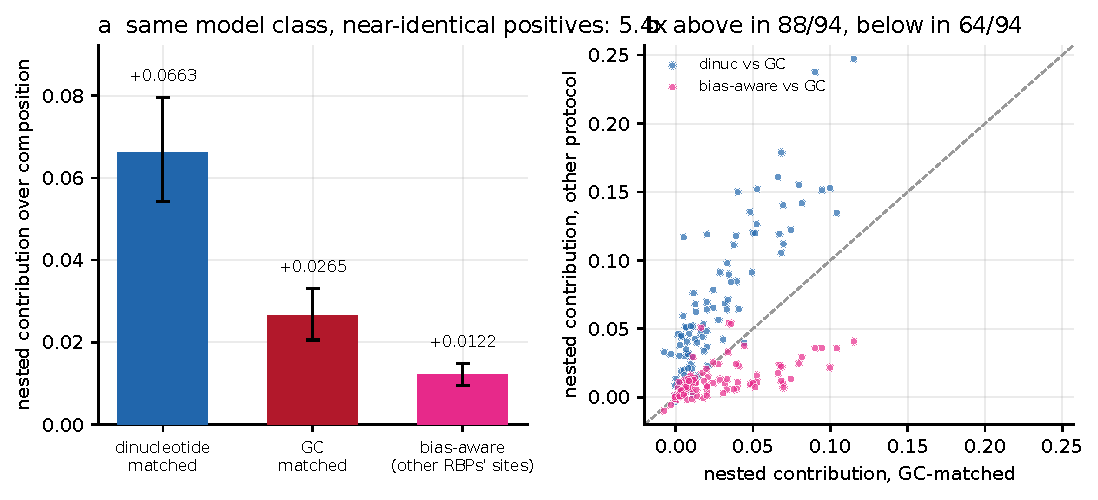
\includegraphics[width=\textwidth]{figures/f10_three_protocols}
\caption{\textbf{The three protocols, and the reversal.} Same 94 datasets, same positives, same 4-mer, same folds and same estimator; only the negatives differ. (a) Composition-only AUROC, apparent AUROC and nested contribution under each protocol. (b) Nested contribution per dataset, dinucleotide-matched against GC-matched, paired; points above the diagonal are the 88 of 94 datasets where the model contributes more under dinucleotide matching. (c) The same for the bias-aware arm against GC-matched, lower in 64 of 94. Apparent AUROC moves in the opposite direction to contribution: dinucleotide matching lowers it in 94 of 94 datasets.}
\label{fig:three}
\end{figure}

\subsection{No rescaling supplies a transportable protocol-free quantity}

AUROC is compressive near one, so a gain measured against a 0.82 baseline is arithmetically
smaller than the same gain against a 0.63 baseline, and part of the 5.42-fold span is scale
rather than protocol. We searched for a coordinate in which the span disappears
(Figure~\ref{fig:scale}).

Over eight monotone reparameterisations of the same 282 protocol-dataset cells, the span falls
but does not close. Somers' $D$ \citep{somers1962} is an affine map of AUROC and returns 5.42 by
construction, which serves as an internal control on the sweep. Every unbounded link reduces the
span, in the order of how aggressively it stretches the upper tail: arcsine 3.99, complementary
log-log 3.94, binormal $d'$ 3.18, logit 2.72. The smallest is obtained by dividing the
contribution by the baseline's own headroom, $1$ minus the composition AUROC, at 2.00
$[1.67, 2.46]$. Normalising instead by the excess over chance, which is the transformation a
reader is most likely to invent, makes the span far worse at 18.2, because the denominator itself
varies with protocol and approaches zero.

The 2.00 figure should not be compared against 1.0. A ratio of the largest to smallest of three
noisy means is bounded below by one and biased upward, so some span is expected under any
sampling. Simulating equal true arm means while preserving the real between-arm dataset pairing
gives a null with median 1.064 and 95th percentile 1.175. The observed 2.00 lies well outside
it, so the residual span is not an artefact of taking a ratio.

The headroom coordinate is not a coordinate, however, but a fitted member of a family, and we
report that rather than resting on it. Dividing by headroom is the $p=1$ case of dividing by
headroom raised to the power $p$, and our sweep stopped at exactly the member we recommend.
Extending the family, the span collapses:

\begin{table}[htbp]
\centering
\caption{Fold span across the three protocols for $g/(1-c)^{p}$, where $g$ is the nested
contribution and $c$ the composition AUROC. An equalising exponent exists in sample.}
\label{tab:exponent}
\begin{tabular}{lccccccc}
\toprule
$p$ & 0 & 0.5 & 1.0 & 1.25 & \textbf{1.544} & 1.75 & 2.0 \\
\midrule
span & 5.42 & 3.43 & 2.00 & 1.48 & \textbf{1.005} & 1.34 & 1.95 \\
\bottomrule
\end{tabular}
\end{table}

At $p=1.544$ the three protocols agree on the panel mean to within 0.5\%. A monotone rescaling
that equalises our three protocols therefore exists, and any claim that none does would be false
on our own data.

The exponent is a property of the benchmark rather than of the quantity, and that is the result.
Fitted to the two negative sets released by \citet{horlacher2023}, the equalising exponent is
3.649, a factor of 2.4 from ours. Our exponent leaves their benchmark at 2.340 against the 2.381
it started from, that is, it buys nothing there. So a normalisation strong enough to equalise one
benchmark must be refitted on the next, and the absence of a protocol-free measure is a
statement about transportability rather than about a floor. Stated that way it is testable, and
we have tested it on data we did not build.

\begin{figure}[htbp]
\centering
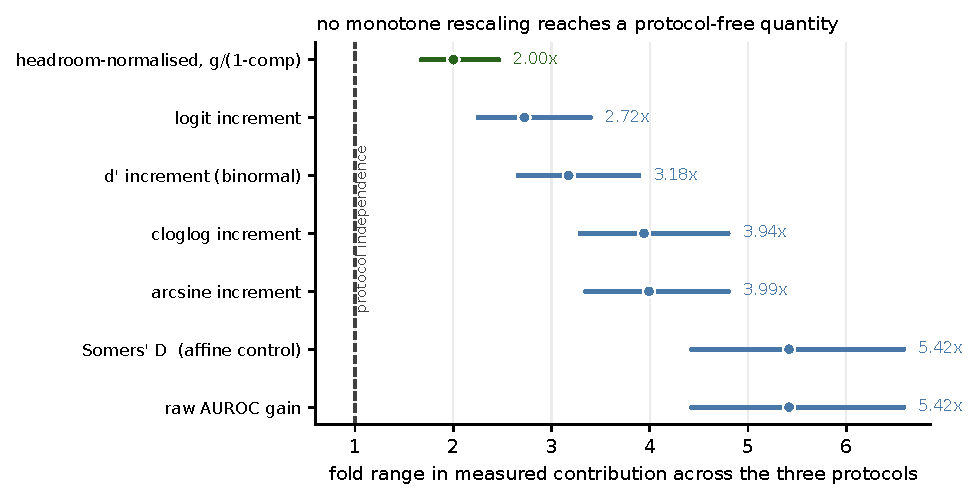
\includegraphics[width=0.72\textwidth]{figures/f11_scale_sweep}
\caption{\textbf{No rescaling reaches a protocol-free quantity among fixed coordinates.} Fold span in measured contribution across the three protocols under eight monotone reparameterisations of the same 282 protocol-dataset cells. Points are the span, bars are 95\% percentile intervals from a bootstrap over datasets (2000 draws), and the dashed line marks protocol independence. Somers' $D$ is an affine map of AUROC and returns the raw value by construction, serving as a control on the sweep. The minimum, 2.00 $[1.67,2.46]$, is attained by dividing by the baseline's own headroom.}
\label{fig:scale}
\end{figure}

\subsection{It is the composition baseline, not the protocol label}

Pooled across all 282 protocol-dataset cells the contribution tracks the composition baseline at
Spearman $-0.600$ ($p=6\times10^{-29}$). We report this as the mechanism rather than defending
against it: most of what a protocol does is decide how much room the baseline leaves. Three
analyses localise the effect (Figure~\ref{fig:baseline}).

\paragraph{Variance accounting.} Regressing the contribution on a cubic in the composition
baseline over all 282 cells and then adding protocol dummies, the protocol label adds 1.0\% of
variance given the baseline, while the baseline adds 11.0\% given the label: an order of
magnitude in the baseline's favour.

\paragraph{A natural experiment.} The bias-aware protocol usually raises the baseline relative
to GC matching, but in 27 of 94 datasets it lowers it. If the protocol label carried the
information, its deficit would persist there. It reverses: $-0.0212$ $[-0.0269, -0.0157]$ where
it raises the baseline, $+0.0028$ $[-0.0000, +0.0063]$ where it lowers it, with within-dataset
Spearman correlation between the change in baseline and the change in contribution of $-0.664$
($p=3\times10^{-13}$). Whichever protocol leaves the lower baseline yields the higher
contribution, regardless of which protocol it is.

\paragraph{Matching on the baseline.} Because the dinucleotide baseline is lower than the GC
baseline in 94 of 94 datasets, arm and baseline are perfectly rank-confounded within a dataset
and the comparison must borrow across datasets. Doing so, the headline $+0.0398$ falls to
$-0.0087$ $[-0.0265, +0.0122]$. We report this and also report why it is not a clean test: the 41
retained pairs are selected from opposing tails, the dinucleotide members having mean baseline
0.6875 against the panel's 0.6274 and the GC members 0.6904 against 0.7827; only 24 distinct GC
partners serve 41 comparisons, with one reused eleven times; and no protein matching is possible.
Nearest-neighbour matching on a variable monotonically related to the outcome, with reuse and
across proteins, is biased toward zero by construction here. The honest reading is that the
comparison is not identified for this pair, which is consistent with the pair's common support
being only 0.073 AUROC wide over 33 of 188 cells.

\paragraph{Where it is identified, a protocol-family residual survives.} The
GC-versus-bias-aware pair overlaps by 0.212 AUROC over 130 of 188 cells, so the same matched
design is straightforward there. Under two independent designs the bias-aware arm still costs
$-0.0081$ $[-0.0130, -0.0036]$ (nearest-baseline matching) and $-0.0043$ $[-0.0077, -0.0012]$
(within-dataset intercept at zero baseline shift). Decomposed by pair, the protocol label's
incremental variance is 0.05\% for GC versus dinucleotide but 3.40\% for GC versus bias-aware, so
the pooled 1.0\% averages a pair where the question is unanswerable with one where it is
answerable.

\paragraph{The mechanism, which changes the framing from three protocols to two families.} The
gradient from baseline to contribution is a property of composition-matched negatives and is
absent otherwise: within-arm Spearman is $-0.545$ (GC), $-0.462$ (dinucleotide) and $-0.122$,
not significant (bias-aware). Inside the composition-matched family the baseline is essentially
the whole story; across families it is not, and a residual of about 0.005 to 0.008 AUROC remains.
This is why we do not name headroom as the general mechanism.

\begin{figure}[htbp]
\centering
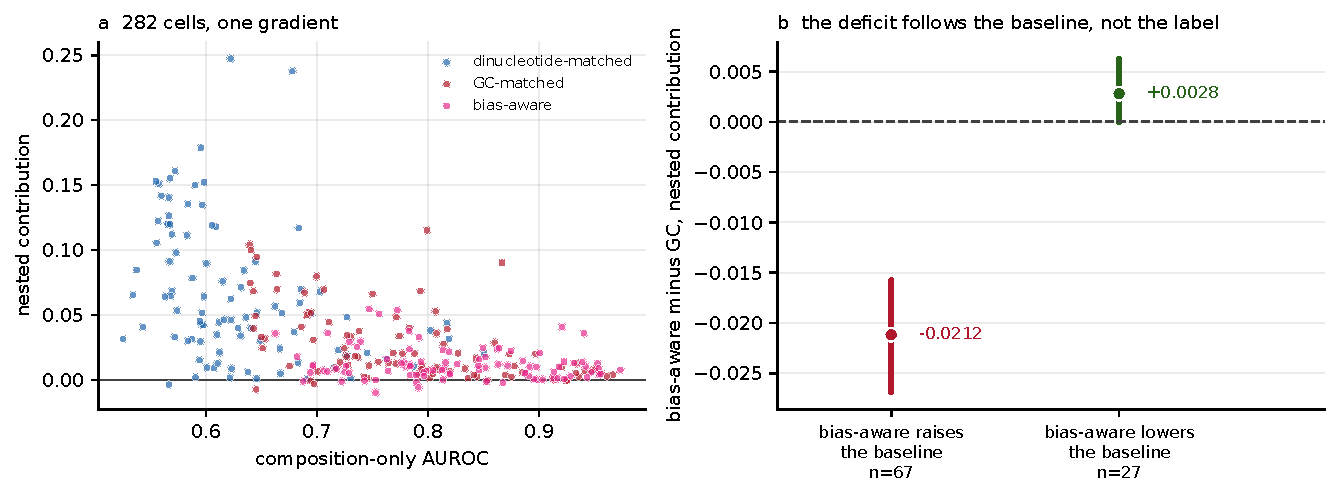
\includegraphics[width=\textwidth]{figures/f12_protocol_or_baseline}
\caption{\textbf{The composition baseline, not the protocol label.} (a) All 282 protocol-dataset cells: nested contribution against the composition-only AUROC the protocol left behind, coloured by protocol; pooled Spearman $-0.600$ ($p=6\times10^{-29}$). (b) The natural experiment. Datasets are split by whether the bias-aware protocol raised or lowered the composition baseline relative to GC matching ($n=67$ and $27$); points are stratum means and bars are 95\% percentile intervals from a bootstrap over datasets (4000 draws). The deficit reverses where the baseline falls.}
\label{fig:baseline}
\end{figure}

\subsection{The effect is not a property of the model class}

The GC arm was swept for two further architectures, 470 fold-runs each: a 7089-parameter
convolutional network in the style of \citet{alipanahi2015} and a fully fine-tuned
19.78~M-parameter SpliceBERT \citep{chen2024}, using the same folds, the same seed and the same
code path, with per-window scores committed (Figure~\ref{fig:models}).

\begin{table}[htbp]
\centering
\caption{The protocol contrast for three model classes, $n=94$ datasets, identical rows and
folds. Intervals are protein-clustered percentile intervals over the 79 proteins.}
\label{tab:models}
\begin{tabular}{lccc}
\toprule
model & GC arm & dinucleotide arm & contrast \\
\midrule
4-mer & $+0.0265$ & $+0.0663$ & $+0.0398$ $[+0.0325, +0.0477]$ \\
CNN & $+0.0330$ & $+0.0860$ & $+0.0530$ $[+0.0440, +0.0627]$ \\
SpliceBERT & $+0.0890$ & $+0.1754$ & $+0.0864$ $[+0.0778, +0.0951]$ \\
\bottomrule
\end{tabular}
\end{table}

The contrast is present for all three model classes on all 94 datasets, which retires the
objection that a five-fold span measured with a bag of $k$-mers is an artefact of a weak model:
it is still a factor of 2.4 for a fine-tuned transformer measured on the same rows.

We then swept both neural models on the bias-aware arm as well, so that the three-protocol
result and the multi-model result meet in the same cells rather than being two separate
two-way comparisons (Table~\ref{tab:threemodels}).

\begin{table}[htbp]
\centering
\caption{The full design: three negative-set protocols by three model classes, $n=94$ datasets,
identical rows and folds throughout. Spans are ratios of panel means with protein-clustered
percentile intervals.}
\label{tab:threemodels}
\begin{tabular}{lcccc}
\toprule
model & dinucleotide & GC & bias-aware & span \\
\midrule
4-mer & $+0.0663$ & $+0.0265$ & $+0.0122$ & 5.42 $[4.43, 6.58]$ \\
CNN & $+0.0860$ & $+0.0330$ & $+0.0113$ & \textbf{7.63} $[6.23, 9.63]$ \\
SpliceBERT & $+0.1754$ & $+0.0890$ & $+0.0466$ & 3.76 $[3.27, 4.34]$ \\
\midrule
composition alone & 0.6274 & 0.7827 & 0.8248 & \\
\bottomrule
\end{tabular}
\end{table}

Three things follow. The span is present for every model class, so it is a property of the
benchmark rather than of the model used to measure it, and the weakest of the three is still
3.76-fold. The bias-aware protocol yields the least for all three models while having the
highest composition baseline, so the reversal in the title is not specific to a $k$-mer. And
the span is \emph{widest for the convolutional network}, not for the largest model, which is the
same non-monotonicity in capacity that the ratio-scale multiplier shows: nothing here grows with
capacity. On the ratio
scale the ordering reverses, the multiplier being 3.08, 3.51 and 2.38 for the three models
(geometric mean over the 77 datasets positive in both arms for all models), so the contrast does
not grow with capacity and we make no such claim.

\paragraph{Whose property is the multiplier?} Decomposing its log over the 262 dataset-by-model
cells where both arms are positive, RBP identity accounts for 64.8\% of the variance, cell line
0.2\% and model class 2.8\%. Those shares are not directly comparable, because a factor with 79
levels absorbs 29.7\% of the variance of relabelled data while a three-level factor absorbs
0.8\%. Measured against a null that permutes protein labels between datasets while keeping each
dataset-by-model block intact, protein's excess is $+7.2$ points ($p=0.003$), and the direct test
is stronger than either share: the same protein's log multiplier agrees across the two cell lines
at $r=0.586$ (Spearman 0.594, $p=0.0001$) over 40 protein-by-model pairs. Cell line is not
detectable, though with only fifteen proteins in both lines the design has little power to
detect it. Model class is small but real ($p=0.023$), consistent with SpliceBERT's significantly
lower multiplier, and it survives the differential censoring visible in its own input.

\paragraph{Why we do not decompose the span into compression and a residual protocol effect.}
The natural next step is to transplant a model's discriminability increment across baselines and
call the unexplained part a protocol effect. That quantity is not identified for any of the three
models. Its central assumption, that the increment is invariant to the baseline it is measured
against, is violated in these data, and across a grid of twelve reasonable specifications only 4
of 6 sign tests hold for the 4-mer, 6 of 6 for the CNN and 1 of 6 for SpliceBERT. One standard
link, the log odds, reverses the sign entirely, which is the behaviour \citet{mood2010} describes
for odds ratios under unobserved heterogeneity. With three arms the transplant residual's sign
follows the direction of transport: carrying an increment from a high-baseline arm to a
low-baseline one gives $+0.0452$ and the reverse gives $-0.0259$. We therefore report the raw
contrast, which needs no transplant, no link and no transportability assumption, and treat the
decomposition as a sensitivity analysis whose failure is itself informative.

\paragraph{A provenance limitation on this section specifically.} For 20 of the 94 datasets in
the dinucleotide arm, the committed neural-network scores were produced under a partition that is
not chromosome-grouped: fold sizes were preserved, so no count-based check detects it, but up to
23 chromosomes appear in a single fold and up to 44.5\% of rows have a same-strand neighbour
within 1~kb assigned to a different fold, against exactly zero under the study folds and zero
throughout the GC arm. The 4-mer is refit on the study folds for every dataset and so is
unaffected, which makes it a clean internal control. Restricting the neural comparison to the 74
correctly partitioned datasets gives contrasts of $+0.0436$ (4-mer), $+0.0506$ (CNN) and
$+0.0878$ (SpliceBERT), all within the protein-clustered interval half-widths of
Table~\ref{tab:models}. We report the 74-dataset figures as primary for the two neural models and
the 94-dataset figures as a sensitivity.

A second asymmetry in the same section, disclosed for completeness: the 4-mer entered the nested
fit as a log odds and the neural models as probabilities, and a logistic regression is not
invariant to a nonlinear transform of a covariate. Refitting the neural arms on the logit scale
raises their contributions by $+0.0008$ (CNN) and $+0.0030$ (SpliceBERT) on the GC arm, so the
published values are conservative, and moves the contrasts by at most 0.0004. AUROC is invariant
to monotone transforms, so no standalone AUROC is affected.

\begin{figure}[htbp]
\centering
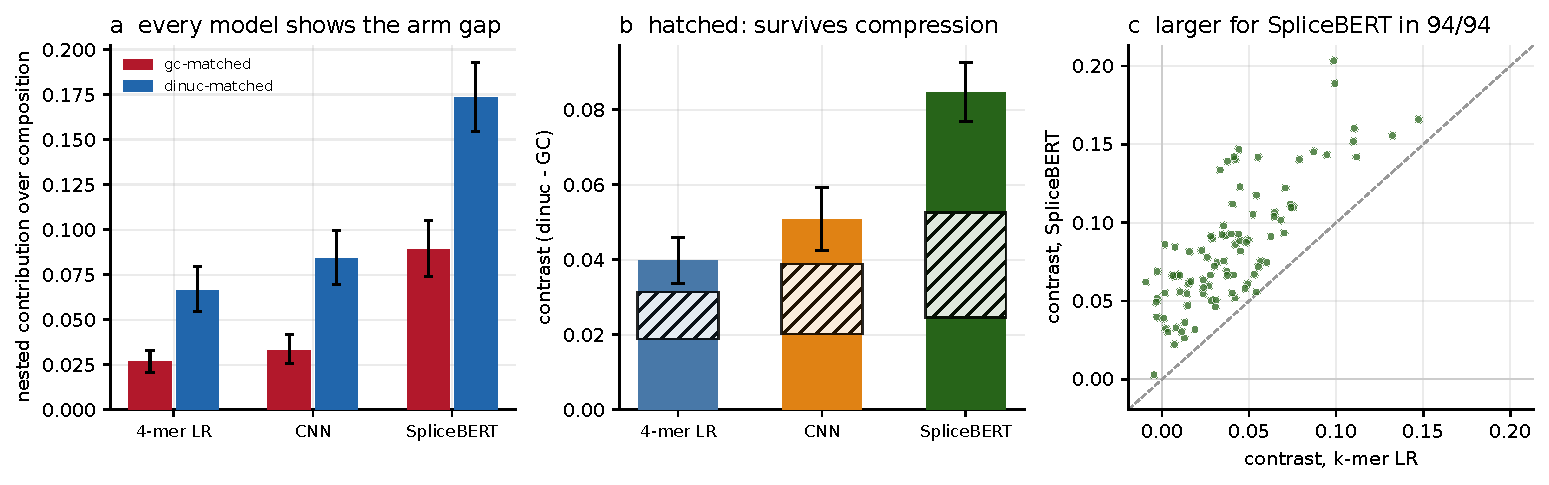
\includegraphics[width=\textwidth]{figures/f9_deep_contrast}
\caption{\textbf{The contrast holds for three model classes.} Nested contribution in each arm for a 4-mer logistic regression, a 7089-parameter convolutional network and a fully fine-tuned 19.78~M-parameter SpliceBERT, on identical rows and folds, $n=94$. Intervals are 95\% percentile intervals from a bootstrap over the 79 proteins, taking all datasets of each sampled protein (4000 draws). On the ratio scale the ordering reverses, so the contrast does not grow with capacity.}
\label{fig:models}
\end{figure}

\subsection{The calibration replicates on an independent benchmark}

Every result above is measured on windows we built. To test whether any of it travels we applied
the identical decomposition to the negative sets released by \citet{horlacher2023}: their
positives, their peak calling, their negative-set construction and their fold assignments, over
the 45 datasets shared with our panel. Only the measurement is ours
(Figure~\ref{fig:external}).

\begin{table}[htbp]
\centering
\caption{The same decomposition on an independent benchmark, $n=45$ datasets. Their positives,
negatives and folds.}
\label{tab:external}
\begin{tabular}{lccc}
\toprule
their negative set & composition & apparent & contribution \\
\midrule
negative-1 (transcript background) & 0.8211 & 0.8606 & $+0.0395$ \\
negative-2 (other RBPs' sites) & 0.7560 & 0.7726 & $+0.0166$ \\
\bottomrule
\end{tabular}
\end{table}

The span on their benchmark is 2.381, against 2.17 for the family-matched pair in our own data,
the GC versus bias-aware comparison; their negative-2 is constructed like our bias-aware arm, so
that is the correct comparison rather than our dinucleotide-versus-GC 2.50.

More importantly, the two-family mechanism replicates arm for arm. The within-arm gradient from
baseline to contribution on their data is $-0.645$ ($p=1.8\times10^{-6}$) for their
composition-matched transcript-background arm and $-0.187$ ($p=0.22$, not significant) for their
other-RBPs'-sites arm, against $-0.545$ and $-0.462$ for our composition-matched arms and
$-0.122$, not significant, for ours. An independent laboratory's negatives and folds reproduce
both the presence of the gradient in one family and its absence in the other.

This also explains the one feature of their benchmark that is anti-monotone to ours: their
negative-2 has both the lower baseline and the lower contribution, which no single-family
headroom relation predicts and which a cross-family residual does.

\begin{figure}[htbp]
\centering
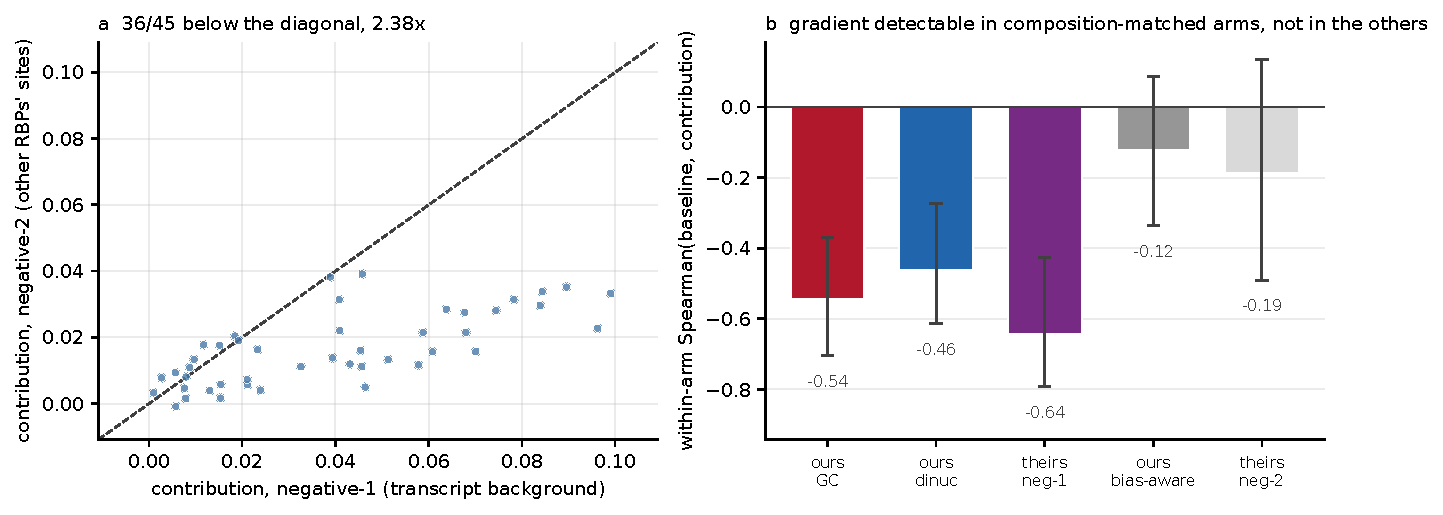
\includegraphics[width=\textwidth]{figures/f14_external_validation}
\caption{\textbf{Replication on an independent benchmark.} \citet{horlacher2023}'s released negative sets, their peak calling and their folds, over the 45 datasets shared with our panel; only the measurement is ours. (a) Nested contribution under their negative-2 against their negative-1, paired per dataset; 36 of 45 fall below the diagonal. (b) The mechanism, which is what travels: the within-arm gradient from composition baseline to contribution, for the composition-matched arms in both benchmarks and the other-RBPs'-sites arms in both. The gradient is present in one family and absent in the other, in both benchmarks independently.}
\label{fig:external}
\end{figure}

\subsection{The recommendation, and the limits of what it buys}

The deliverable is a two-number report: state the composition-only AUROC obtained under the same
protocol beside every headline AUROC. Everything above shows that not doing so is a problem.
Whether doing so helps is a separate question, and we tested it by putting a reader in the
position the recommendation is meant to rescue, holding two papers that used different protocols
and wanting to compare what the models contributed (Figure~\ref{fig:recommendation}).

On our data, normalising by headroom improves rank agreement in 3 of 3 protocol pairs and reduces
disagreement on a common scale in 3 of 3, by 58\%, 10\% and 48\%. Rank agreement is scale-free,
so no normalisation can flatter it.

Two findings qualify this. First, only the GC-versus-dinucleotide rank improvement has an
interval clear of zero ($+0.051$ $[+0.007, +0.115]$); the other two pairs are consistent in
direction and individually null. That pair is precisely the one where the protocol label adds
0.05\% of variance, so the fix is best demonstrated where it is least needed. Second, and
decisively, the test fails to replicate out of sample. On the 45 datasets of
\citet{horlacher2023}, rank agreement \emph{falls} from 0.706 to 0.656 under normalisation and
disagreement \emph{rises} from 0.860 to 0.908. Those are, verbatim, the two criteria we
pre-registered as falsifying. The change in rank agreement is $-0.050$ $[-0.222, +0.140]$, so at
$n=45$ this is a failure to replicate rather than a refutation, but it points the wrong way and
we report it.

We therefore make the weaker claim that the evidence supports. Report the composition-only AUROC
under the same protocol, because it is the only summary of what the protocol did that a reader
can act on and because it makes the problem visible. Do not treat any normalisation as making
contributions comparable across protocols: we cannot demonstrate that it does, and on
independent data it does not. The operational recommendation is to report the baseline and to
refrain from cross-protocol comparison, not to rescale and proceed.

\begin{figure}[htbp]
\centering
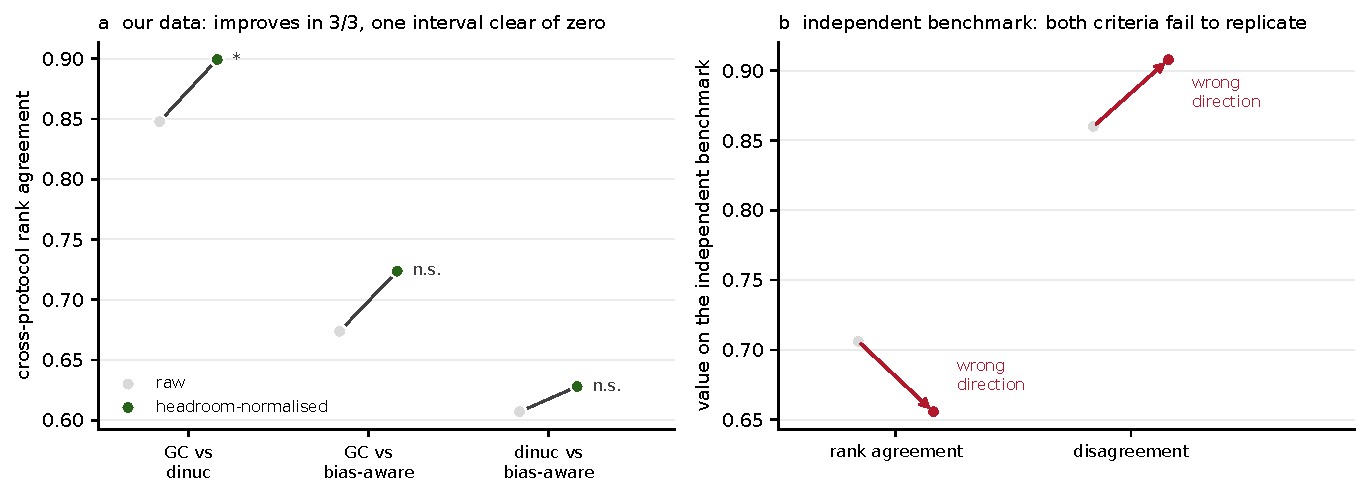
\includegraphics[width=\textwidth]{figures/f15_recommendation}
\caption{\textbf{The recommendation, and where it stops working.} (a) On our data, cross-protocol rank agreement before and after dividing by the baseline's headroom, for each protocol pair. Agreement improves in 3 of 3, but only the GC-versus-dinucleotide improvement has a protein-clustered interval clear of zero. (b) The same test on the independent benchmark of Figure~\ref{fig:external}, $n=45$: rank agreement falls and disagreement rises under normalisation, which are the two criteria pre-registered as falsifying the recommendation. The change in rank agreement is $-0.050$ $[-0.222,+0.140]$, so this is a failure to replicate rather than a refutation.}
\label{fig:recommendation}
\end{figure}
